\documentclass[../main.tex]{subfiles}
\graphicspath{{\subfix{../images/}}}
\begin{document}
\section{Entwicklung}

\subsection{Hardware}
\subsubsection{Bridge}
Zur Entwicklung der Verbindungsplatine wurde die Hardware zunächst auf einem Breadboard aufgesteckt und eine geeignete Verbindung der notwendigen Pins mithilfe ausreichender Steckbrückenkabel hergestellt und umfangreich getestet. Anschließend wurde der Schaltplan nach Vorlage des Breadboards in KiCad Version 7.0 erstellt, woraus sich im weiteren Verlaufe ein Leiterplattenentwurf erstellen ließ. Der Druck der Leiterplatte erfolgte auf Anfrage im KI-Labor am Umwelt-Campus Birkenfeld.

\begin{figure}[!ht]
    \centering
    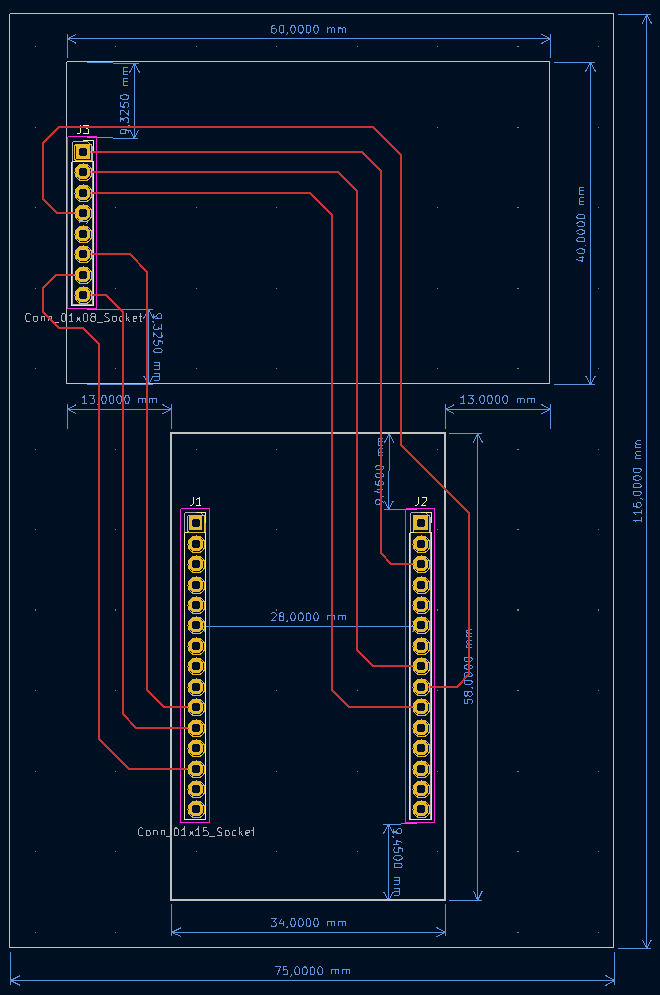
\includegraphics[width=0.4\textwidth, angle=-90]{images/leiterplatte.png}
    \caption{Leiterplattenplan aus dem Leiterplatteneditor der Software KiCad 7}
    \label{fig:Bridge}
    \centering
\end{figure}



\subsubsection{Hülle}

Das Gehäuse wurde innerhalb von Fusion 360 designt und dann mit PLA Filament 3D gedruckt. Es hat mehrere Anläufe gebraucht um das richtige Design hinzubekommen.

\begin{figure}[!ht]
    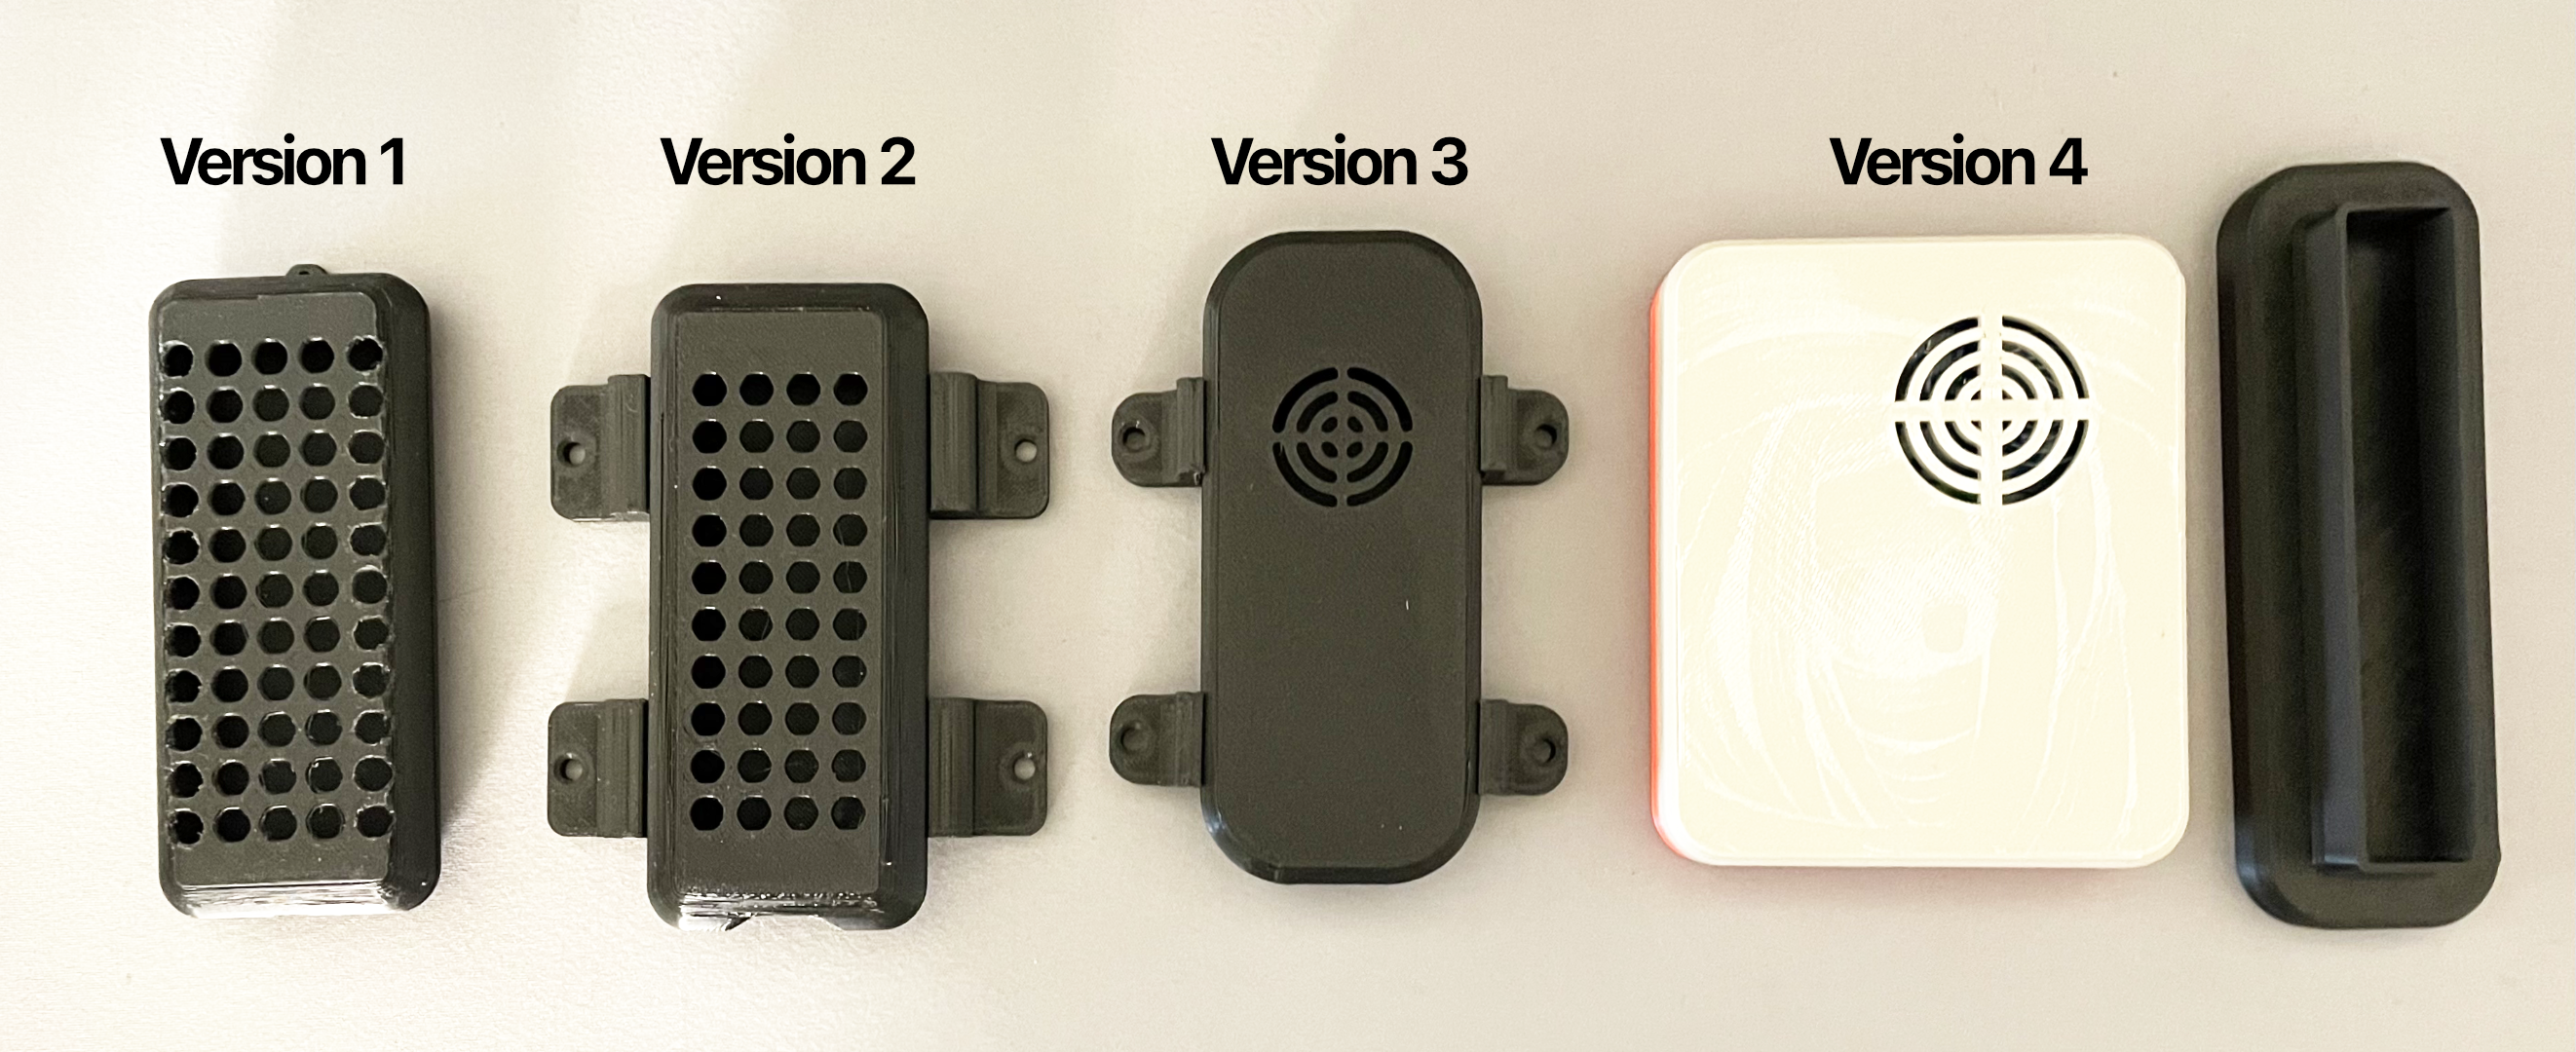
\includegraphics[width=\linewidth]{images/huellen_versionen.png}
    \caption{Alle Versionen des Hüllen Designs}
    \centering
\end{figure}

\subsection{API Design} \label{JSON-API}

Zur Erstellung unseres Systems haben wir uns auf folgende JSON Struktur geeinigt, um die Daten zwischen den verschiedenen Softwaresystemen zu kommunizieren. 

\begin{lstlisting}
{
    "key": "api key",
    "data": {
        "request_data": "Some Data"
    },
    "error": "Error Message"
}
\end{lstlisting}

\begin{itemize}
  \item\textbf{Key}: Das Key Attribut enthält den API-Schlüssel, welcher das System schützt vor nicht autorisierten Zugriffen.
  \item\textbf{Data}: Ist ein weiteres JSON Objekt innerhalb der Abfrage, welches Abfragen spezifische Daten enthält.
  \item\textbf{Error}: Error enthält den Text einer entstandenen Fehlermeldung.
\end{itemize}

\subsection{Benutzeroberfläche}
\begin{itemize}
  \item Menüsystem, Bildschirme gestalten.
\end{itemize}

\subsection{Benutzerverwaltung/Authentifizierung}
\begin{itemize}
  \item Funktionen für Erstellung, NFC-Reading/Writing, Authentifizierung entwickeln.
\end{itemize}

\subsection{Zeiterfassung} \label{ZeitwerfassungEntwicklung}
Zunächst wurden Nachforschungen betrieben, welche Möglichkeiten es gibt um eine zuverlässige Erfassung der Zeit zu gewährleisten. Neben diversen hardwarebasierten Erfassungsmethoden fiel Wahl schließlich auf eine softwarebasierte Erfassung. Dies umfasst die Zeitanfrage über eine Anfrage an einen Network Time Protocol Server.\\
Der Vorteile der sich hieraus ergibt ist, dass keine weitere Hardware benötigt wird um die Zeit zu erfassen.\\ 
Der größte Nachteil dieser Methode ist jedoch, dass zwangsläufig eine Netzwerkverbindung bestehen muss, um die Zeit vom NTP Server erhalten zu können.
\subsubsection{Unix Epoch Time} 
Die Zeit wird hierbei lediglich als Unix Timestamp, also der Anzahl an vergangenen Sekunden seit dem 1. Januar 1970, 00:00 Uhr UTC, erfasst und an den Server weitergegeben, da die Zeit dadurch einfach als Integer in der Datenbank hinterlegt werden kann. Hier kommt es jedoch zu Komplikationen der Zeiterfassung am 19. Januar 2038, da unsere Datenbank lediglich 32-Bit Integer speichert.


\subsection{Datenanzeige}
\begin{itemize}
  \item Funktionen für Berichte und Benutzerdaten erstellen.
\end{itemize}

\subsection{Sicherheit}
\begin{itemize}
  \item Verschlüsselung, sichere Datenbehandlung sicherstellen.
\end{itemize}

\subsection{Protokollierung/Prüfung}
\begin{itemize}
  \item Funktionen für Protokollierung und Prüfung entwickeln.
\end{itemize}
\end{document}